\documentclass[11pt]{article}

\usepackage[margin=1in]{geometry}
\usepackage{booktabs}
\usepackage{tabularx}
\usepackage{longtable}
\usepackage{array}
\usepackage{graphicx}
\usepackage{subcaption}
\usepackage{amsmath, amssymb}
\usepackage{hyperref}
\usepackage{xcolor}
\usepackage{enumitem}
\usepackage{tikz}
\usepackage{pgfplots}
\usepackage{verbatim}
\usetikzlibrary{arrows.meta, positioning, shapes.geometric, calc}
\pgfplotsset{compat=1.18}

\newcommand{\method}[1]{\texttt{#1}}
\newcommand{\code}[1]{\texttt{#1}}

\title{HeLMAS-3n: Nested-State Uplift for Gemma 3n E4B}
\author{Draft for PhD review}
\date{\today}

\begin{document}
\maketitle

\begin{abstract}
This paper focuses on HeLMAS-3n: nested-state uplift inside a single Gemma 3n E4B checkpoint. The active question is whether a low-activation nested regime can be translated into the full-activation regime well enough to recover continuation behavior after handoff. We study paired low/full forward passes on identical prompt prefixes, extract matched residual-stream states and caches, and train lightweight translators that approximate full-regime state from low-regime state. Across completed pilot, layer-sweep, suffix-span, and targeted-site experiments, the low/full regimes are clearly separated, identity control is exact, and the best learned intervention site is a specific full-regime patch surface at
\method{layer34,last1}. A broader MLP baseline improves local state alignment but dilutes the site-specific continuation effect. The current evidence therefore points to intervention placement, not raw model capacity, as the dominant bottleneck.
\end{abstract}

\tableofcontents
\newpage

\section{Introduction}
HeLMAS-3n studies same-parent-model handoff inside Gemma 3n E4B. The aim is practical and falsifiable: recover full-regime continuation behavior from low-regime prefix state using a lightweight uplift map.

HeLMAS-3n deliberately narrows the question. Gemma 3n E4B is designed around a nested / MatFormer-style structure with selective activation and dynamic resource usage \cite{gemma3n2025,mrl2022}. That makes it a better testbed for a same-parent-state uplift hypothesis: the low-activation regime is not an alien model, but a compressed sibling of the full regime. If the sibling relation is real, the translation from low to full should be a small corrective map rather than a universal bridge.

The paper therefore asks a limited question:
\begin{quote}
Can a low-activation Gemma 3n E4B prefix state be uplifted into the corresponding full-activation state so that decoding resumes closer to native full-regime behavior?
\end{quote}

This draft is conservative. It includes only completed results and explicitly labels the larger held-out80 rerun as active validation.

\section{Historical context (brief)}
The repository includes archived material from an earlier heterogeneous He-LMAS bridge attempt \cite{helmasLegacy2026}. That line remains useful as context but is not the active research track.

The current track is HeLMAS-3n: same-checkpoint regime uplift in Gemma 3n E4B \cite{gemma3n2025}. The key framing change is:
\begin{itemize}[leftmargin=1.4em]
    \item Archived He-LMAS: cross-model transfer.
    \item HeLMAS-3n: same-parent regime uplift.
\end{itemize}
This narrower formulation is what made the current experiments falsifiable.

\section{Method}
\subsection{Paired-state extraction}
For each prompt prefix we run the same checkpoint twice: once under the low regime and once under the full regime. The extraction pipeline stores matched metadata and states at aligned token positions and layers.

The stored sample schema includes:
\begin{itemize}[leftmargin=1.4em]
    \item prompt id
    \item token position
    \item layer index
    \item residual-stream state in low and full regimes
    \item optional KV cache slices
    \item optional sparse logits snapshots
\end{itemize}

The extraction scripts use absolute path resolution and write sharded artifacts with manifest files. That detail matters because the run history showed that path ambiguity can silently truncate the held-out split.

\subsection{Targets}
The primary target is the residual-stream state. The KV cache is retained as a secondary comparison target.

We do this intentionally. If residual uplift works, the full regime's own projection layers can generate the relevant K and V states. Direct KV uplift is therefore a stricter and more brittle target, and it should only be promoted after residual uplift is established.

\subsection{Models}
We evaluate four families of translators:
\begin{itemize}[leftmargin=1.4em]
    \item \method{identity}: no correction.
    \item \method{mean-delta} and linear variants: minimal parametric baselines.
    \item \method{lowrank} and \method{mlp}: small learned translators.
    \item \method{flow}: a placeholder for future refinement, not the first-stage solution.
\end{itemize}

The current paper focuses on the residual target. KV uplift is tracked but not elevated above the residual result until it proves useful.

\subsection{Handoff evaluation}
The central evaluation is resumed decoding after handoff. We use greedy continuation metrics with horizons 1, 4, 8, and 16 tokens. The same prompt prefix is used in both regimes; the low-regime state is patched, and decoding then resumes under the full regime.

Our metric ladder is:
\begin{enumerate}[leftmargin=1.4em]
    \item local state match (cosine / MSE)
    \item next-token agreement / KL proxy
    \item short continuation match after handoff
    \item longer-horizon drift
\end{enumerate}

The project only counts as successful when the lower rung improves and the continuation rung improves as well.

\subsection{Controls and failure gates}
The strictest control is the identity row. Identity must match proper low-to-full no-patch exactly.

Other gates used in the run sequence:
\begin{itemize}[leftmargin=1.4em]
    \item low/full separation must be meaningful before training anything.
    \item extractor pairing must be unambiguous at the prompt/layer/token level.
    \item learned translation must beat the proper no-patch baseline before any architectural escalation.
    \item oracle patch rows are reference patches, not ceilings.
\end{itemize}

\subsection{Experimental path}
Figure~\ref{fig:pipeline} summarizes the active research path.

\begin{figure}[h]
    \centering
    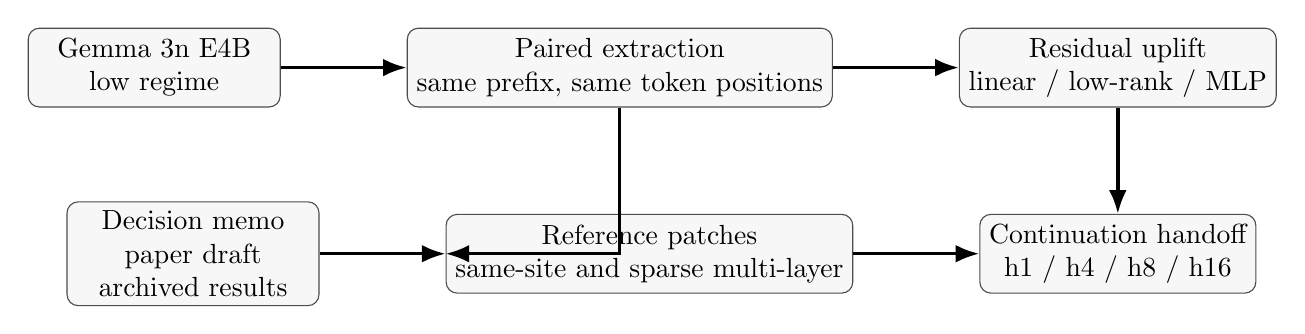
\begin{tikzpicture}[
        node distance=1.35cm and 1.6cm,
        box/.style={rounded corners, draw=black!70, fill=black!3, align=center, minimum width=3.2cm, minimum height=1cm},
        arrow/.style={-{Latex[length=3mm]}, very thick}
    ]
        \node[box] (src) {Gemma 3n E4B\\low regime};
        \node[box, right=of src] (pair) {Paired extraction\\same prefix, same token positions};
        \node[box, right=of pair] (train) {Residual uplift\\linear / low-rank / MLP};
        \node[box, below=of train] (eval) {Continuation handoff\\h1 / h4 / h8 / h16};
        \node[box, left=of eval] (oracle) {Reference patches\\same-site and sparse multi-layer};
        \node[box, left=of oracle] (paper) {Decision memo\\paper draft\\archived results};

        \draw[arrow] (src) -- (pair);
        \draw[arrow] (pair) -- (train);
        \draw[arrow] (train) -- (eval);
        \draw[arrow] (oracle) -- (eval);
        \draw[arrow] (paper) -- (oracle);
        \draw[arrow] (pair) |- (oracle);
    \end{tikzpicture}
    \caption{HeLMAS-3n research pipeline. The current evidence comes from paired extraction, local uplift training, and continuation handoff evaluation.}
    \label{fig:pipeline}
\end{figure}

\section{Experiment chronology}
Table~\ref{tab:timeline} records the actual sequence of experiments and the gate each one answered.

\begin{table}[h]
    \centering
    \small
    \begin{tabularx}{\textwidth}{>{\raggedright\arraybackslash}p{0.18\textwidth}X>{\raggedright\arraybackslash}p{0.26\textwidth}}
\toprule
Phase & What was tested & Outcome \\
\midrule
0 & Low/full separation sanity check & Passed: the two regimes are meaningfully different. \\
1 & Extractor validation on structured prompts & Passed: paired residuals, caches, and logits line up. \\
2 & Null controls plus broad baseline table & Passed: identity equals no-patch; broad MLP is not enough. \\
3 & Layer sweep over candidate sites & Passed: layer 34 is the strongest learned site. \\
4 & Suffix-span sweep at the selected sites & Passed: last1 is already the informative span. \\
5 & Targeted study with held-out prompts & Passed: layer34,last1 generalizes; oracle is reference. \\
6 & Held-out80 rerun with fail-fast checks & Completed: 80 prompts loaded and evaluated. \\
\bottomrule
\end{tabularx}

    \caption{Experiment chronology and the question each run answered.}
    \label{tab:timeline}
\end{table}

\section{Results}
\subsection{Core targeted-site result}
The strongest completed result is the targeted site study. The initial broad MLP baseline improved local alignment, but it was the targeted residual translator at \method{layer34,last1} that generalized most clearly on held-out prompts.

\begin{table}[h]
    \centering
    \small
    \caption{Continuation match versus full-regime decoding for the frozen targeted site study. Values are exact means over the completed pilot and held-out-10 splits.}
    \begin{tabular}{lcccccccc}
\toprule
Method & Pilot h1 & Pilot h4 & Pilot h8 & Pilot h16 & Held-out h1 & Held-out h4 & Held-out h8 & Held-out h16 \\
\midrule
No patch & 0.000000 & 0.006250 & 0.009375 & 0.012500 & 0.000000 & 0.000000 & 0.000000 & 0.006250 \\
Identity & 0.000000 & 0.006250 & 0.009375 & 0.012500 & 0.000000 & 0.000000 & 0.000000 & 0.006250 \\
Broad MLP & 0.000000 & 0.012500 & 0.021875 & 0.017188 & 0.000000 & 0.000000 & 0.012500 & 0.012500 \\
Targeted MLP @ layer16 & 0.000000 & 0.006250 & 0.009375 & 0.010937 & 0.000000 & 0.000000 & 0.000000 & 0.000000 \\
Targeted MLP @ layer34 & 0.825000 & 0.212500 & 0.115625 & 0.067187 & 0.700000 & 0.175000 & 0.100000 & 0.056250 \\
Oracle layer16 & 0.000000 & 0.012500 & 0.021875 & 0.017188 & 0.000000 & 0.000000 & 0.000000 & 0.000000 \\
Oracle layer34 & 0.250000 & 0.068750 & 0.037500 & 0.028125 & 0.400000 & 0.100000 & 0.050000 & 0.031250 \\
Oracle stride & 0.200000 & 0.081250 & 0.046875 & 0.031250 & 0.300000 & 0.075000 & 0.050000 & 0.025000 \\
\bottomrule
\end{tabular}

    \label{tab:core}
\end{table}

\begin{figure}[h]
    \centering
    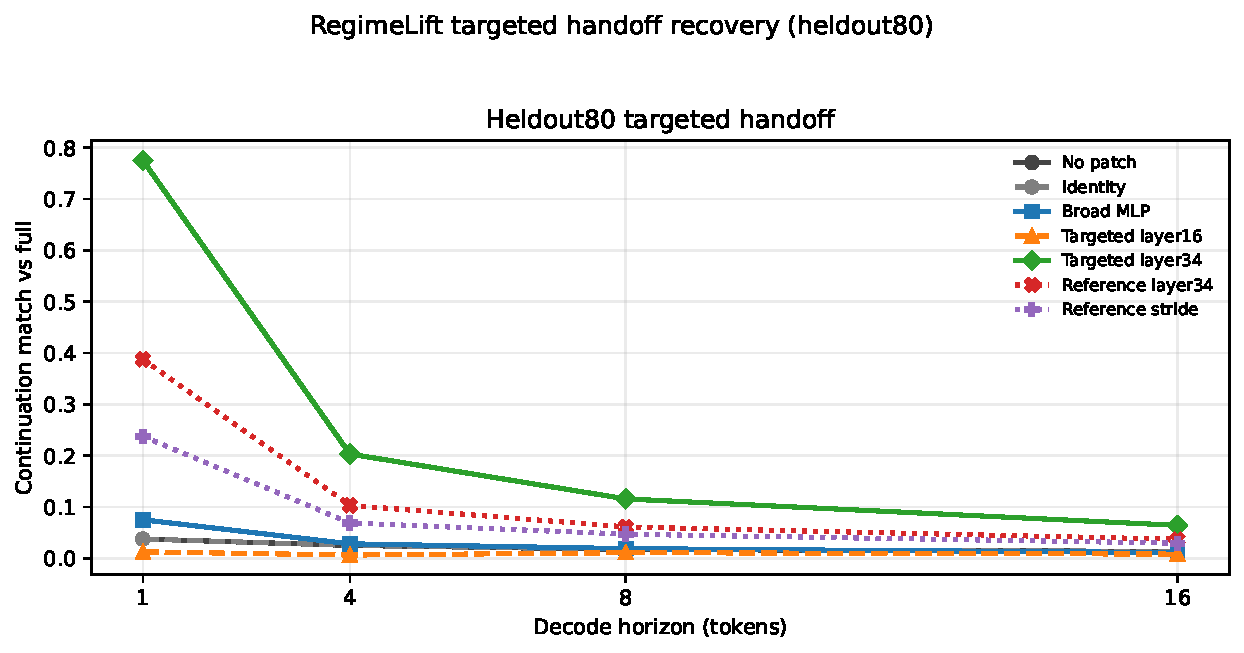
\includegraphics[width=0.95\linewidth]{figures/targeted_handoff_curves.pdf}
    \caption{Continuation match curves for the targeted site study. The plot shows why \method{layer34,last1} became the stable learned site: it is the first row that clearly improves held-out continuation recovery instead of only local state fit.}
    \label{fig:targeted-curves}
\end{figure}

The important read on Table~\ref{tab:core} and Figure~\ref{fig:targeted-curves} is not just that the learned translator beats no-patch. It is that the learned translator at the correct site beats the broad baseline by enough to survive a held-out split.

\subsection{Layer sensitivity}
The layer sweep showed that site choice matters more than raw model capacity. The strongest learned continuation signal does not appear everywhere; it concentrates at specific layers. In particular, \method{layer16} looked promising early, but it was not robust once the controls were corrected and held-out prompts were enforced.

\begin{table}[h]
    \centering
    \small
    \begin{tabular}{lcccc}
\toprule
Method & Best layer @ h8 & h8 & Best layer @ h16 & h16 \\
\midrule
identity & 0 & 0.009375 & 0 & 0.012500 \\
mlp & 16 & 0.021875 & 4 & 0.020313 \\
oracle\_full\_state & 34 & 0.037500 & 34 & 0.028125 \\
\bottomrule
\end{tabular}

    \caption{Summary of the corrected layer sweep. The table reports the best layer for horizon 8 and horizon 16 for each method family.}
    \label{tab:layersweep}
\end{table}

\begin{figure}[h]
    \centering
    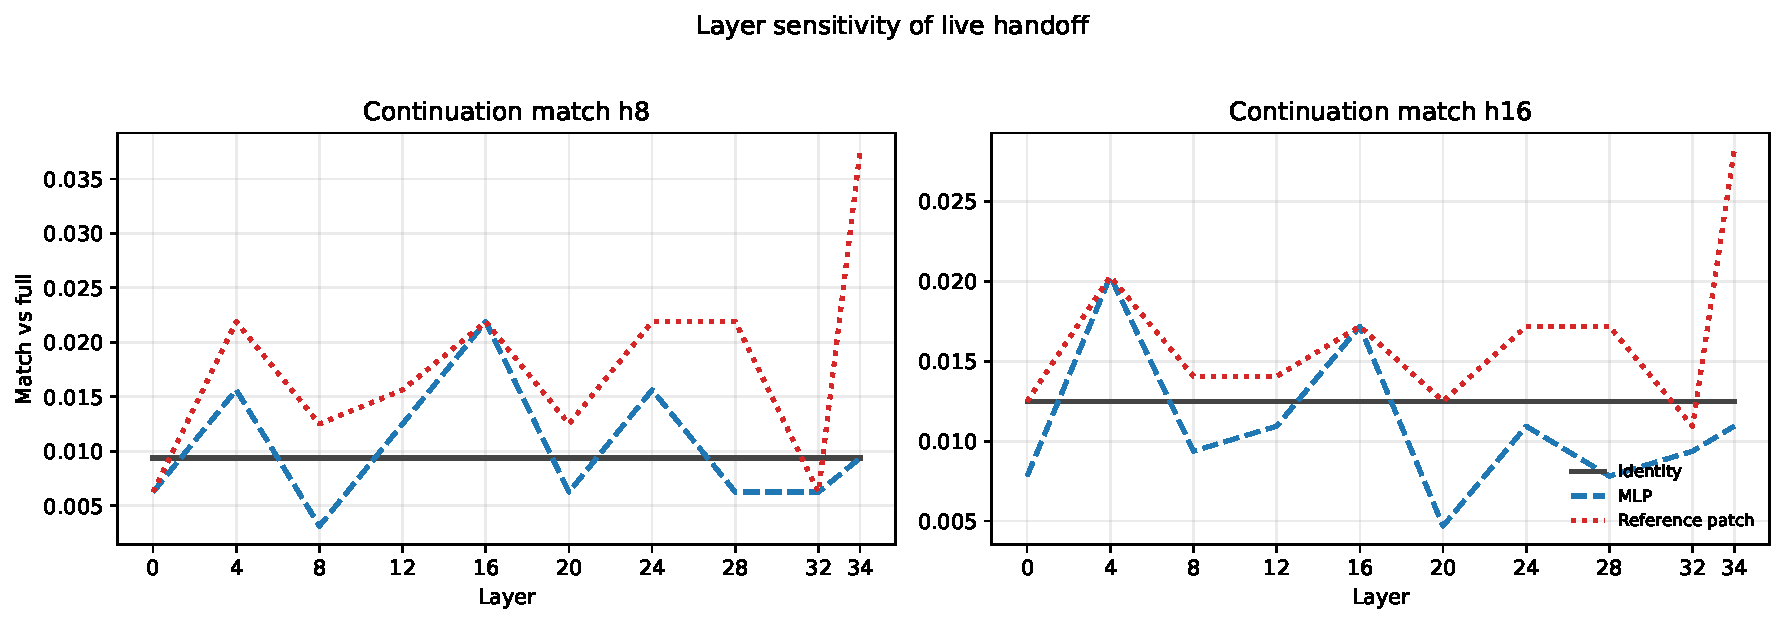
\includegraphics[width=0.95\linewidth]{figures/layer_sweep_sensitivity.pdf}
    \caption{Layer sensitivity for live handoff. The learned translator and the reference patch peak at different layers, but the same conclusion remains: continuation recovery is controlled by a narrow intervention surface rather than a uniformly good translator.}
    \label{fig:layersweep}
\end{figure}

\subsection{Suffix-span sensitivity}
The suffix-span sweep addressed a narrower question: does the patch need more recent context than the last token? The answer in the completed pilot was mostly no. Once the intervention surface was at the right site, widening the suffix from last 1 to last 4 or last 8 tokens did not buy much in the measured continuation metrics.

\begin{figure}[h]
    \centering
    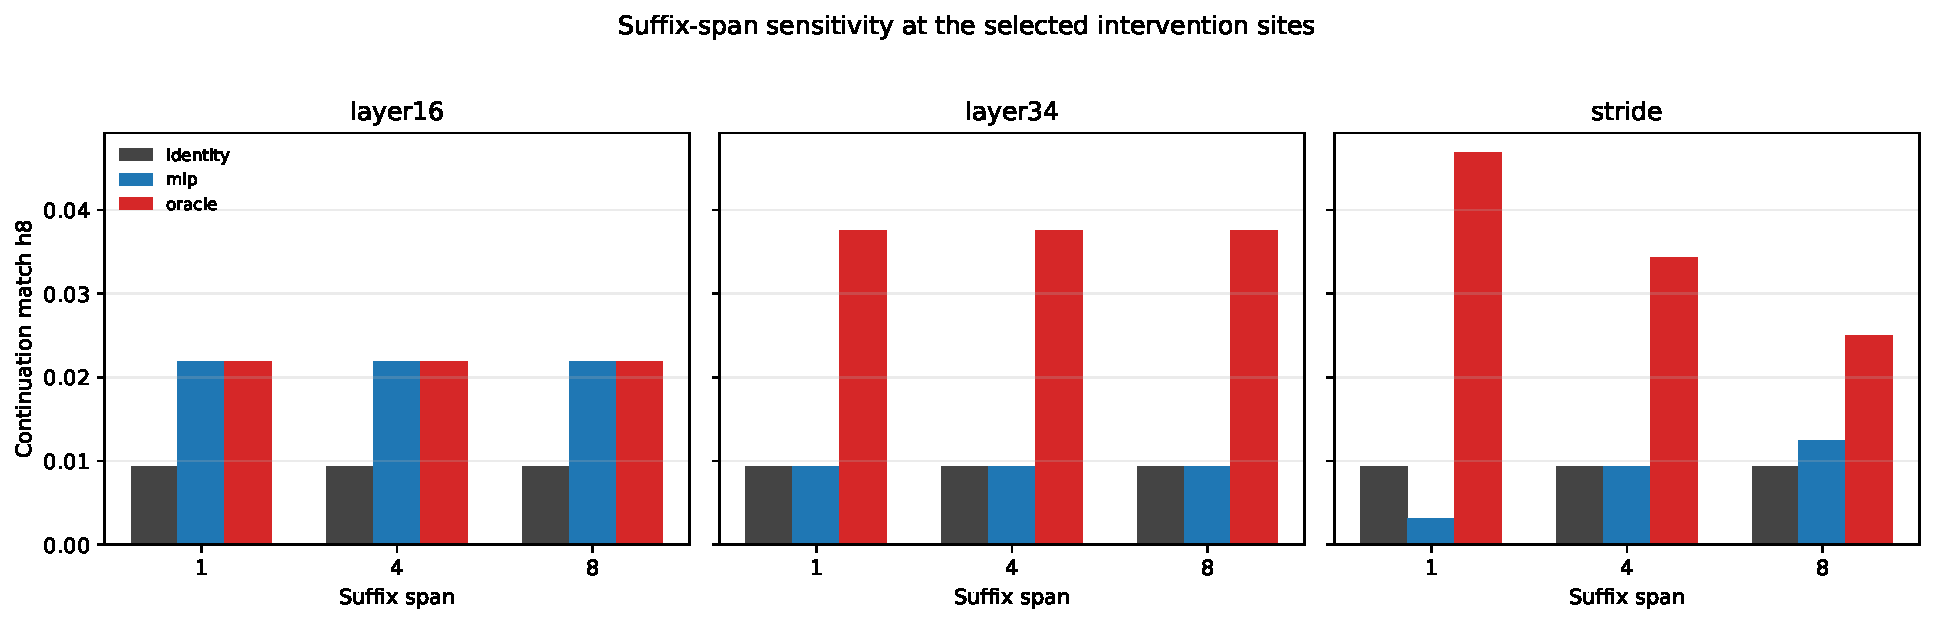
\includegraphics[width=0.95\linewidth]{figures/suffix_span_sensitivity.pdf}
    \caption{Suffix-span sensitivity at the selected intervention sites. The main signal is that the patch width is not the dominant knob once the site is correct.}
    \label{fig:suffix}
\end{figure}

\subsection{What the evidence supports}
The current evidence is strong enough to support the following claims:
\begin{itemize}[leftmargin=1.4em]
    \item low/full regimes in Gemma 3n E4B are genuinely different;
    \item identity is a correct control and equals proper no-patch;
    \item learned uplift is real but site-dependent;
    \item \method{layer34,last1} is the first learned site that generalizes on held-out prompts;
    \item oracle rows are reference patches, not strict ceilings;
    \item the dominant bottleneck is intervention placement, not just translator width.
\end{itemize}

\section{Discussion}
\subsection{Why the result changed the project}
The project started as a question about whether a model can recover another model's reasoning path. The completed experiments show that the answer depends strongly on the intervention surface. A broad MLP can make state vectors look better, but that is not the same as recovering continuation behavior.

This matters scientifically because it shifts the center of gravity from "bigger translator" to "where does the correction land?" That is a more causal and more publishable question.

\subsection{Why \method{layer34,last1} matters}
The completed targeted-site study and the held-out validation both point to one site: \method{layer34,last1}. This is the first site where the learned model is not merely a prettier fit. It is a practical handoff site.

The companion lesson is equally important: \method{layer16,last1} was a false lead. It looked plausible in earlier sweeps, but it did not survive the more disciplined evaluation.

\subsection{Why the oracle is a reference patch, not a ceiling}
At least one learned row beats the same-site oracle on some horizons. That means the exact-substitution reference patch is not a behavioral upper bound. The likely reasons are non-monotonicity in the continuation metric, operational mismatch between exact substitution and the learned patch, or the fact that raw fidelity is not identical to optimal rollout behavior.

The paper therefore uses the label ``reference patch'' instead of ``upper bound''.

\subsection{Current limitation}
The active held-out80 rerun is still in flight. That run exists because the earlier held-out validation accidentally used only 10 prompts. The current evaluator now hard-fails on prompt-count mismatch and writes incremental artifacts so that future failures leave usable evidence.

This is a run-hygiene fix, not a research-direction change.

\section{Log excerpts and run audit}
The following excerpts are included to document how the current active run was actually executed.

\subsection{Held-out80 gate}
\begin{verbatim}
"resolved_heldout_extract_config": "/home/marcel/Work/He-LMAS/helmas3n/configs/extract_killtest40_holdout80.yaml"
"resolved_heldout_prompts_path": "/home/marcel/Work/He-LMAS/data/prompt_pool_v1_holdout80.jsonl"
"heldout_prompt_count": 80
"heldout_prompt_id_first": "sym_0253"
"heldout_prompt_id_last": "con_0079"
[targeted] split=heldout prompts=80
\end{verbatim}

\subsection{Interpretation-excerpt}
\begin{verbatim}
Identity control passed.
layer34,last1 is the useful learned site.
layer16,last1 is not robust enough to carry forward.
\end{verbatim}

\section{Conclusion}
HeLMAS-3n is no longer a speculative bridge idea. It is a measured regime-uplift problem inside Gemma 3n E4B with a stable experimental spine:
\begin{itemize}[leftmargin=1.4em]
    \item the low/full regimes differ;
    \item the control path is sound;
    \item \method{layer34,last1} is the first practical learned handoff site;
    \item broad translators are not enough by themselves;
    \item continuation recovery is controlled by a narrow intervention surface.
\end{itemize}

The next step is to finish the held-out80 validation, then decide whether to refine the objective at the same site or promote the project to the KV target.

\bibliographystyle{plain}
\bibliography{references}

\end{document}
